%! TeX program = lualatex
\documentclass[a4paper]{article} 

% packages
\usepackage{microtype}      % Slightly tweak font spacing for aesthetics
\usepackage[english]{babel} % Language hyphenation and typographical rules
\usepackage[final, colorlinks = true, urlcolor = black, linkcolor = black]{hyperref} 
\usepackage{changepage}     % adjust margins on the fly

\usepackage{fontspec}
\setmainfont{EB Garamond}
\setmonofont[Scale=MatchLowercase]{Deja Vu Sans Mono}

\usepackage{minted}
\usemintedstyle{algol_nu}
\usepackage{xcolor}

\usepackage{pgfplots}
\pgfplotsset{width=\textwidth,compat=1.9}

\usepackage{caption}
\newenvironment{code}{\captionsetup{type=listing}}{}
\captionsetup[listing]{skip=0pt}
\setlength{\abovecaptionskip}{5pt}
\setlength{\belowcaptionskip}{5pt}

\usepackage[yyyymmdd]{datetime}
\renewcommand{\dateseparator}{--}

\usepackage{titlesec}
% \titleformat{\section}{\LARGE\bfseries}{}{}{}[\titlerule]
% \titleformat{\subsection}{\Large\bfseries}{}{0em}{}
% \titlespacing{\subsection}{0em}{-0.7em}{0em}
%
% \titleformat{\subsubsection}{\large\bfseries}{}{0em}{$\bullet$ }
% \titlespacing{\subsubsection}{1em}{-0.7em}{0em}

% margins
\addtolength{\hoffset}{-2.25cm}
\addtolength{\textwidth}{4.5cm}
\addtolength{\voffset}{-3.25cm}
\addtolength{\textheight}{5cm}
\setlength{\parskip}{0pt}
\setlength{\parindent}{0in}
% \setcounter{secnumdepth}{0}

\begin{document}
\hrule \medskip
\begin{minipage}{0.295\textwidth} 
    \raggedright
    \footnotesize 
    \begin{tabular}{@{}l l} % Define a two-column table with left alignment
        Name: & Andrew Hayes \\
        Student ID: & 21321503 \\
    \end{tabular}
\end{minipage}
\begin{minipage}{0.4\textwidth} 
    \centering 
    \vspace{0.4em}
    \LARGE 
    \textsc{ct404} \\ 
\end{minipage}
\begin{minipage}{0.295\textwidth} 
    \raggedleft
    \footnotesize 
    \begin{tabular}{@{}l l} % Define a two-column table with left alignment
        Name: & Cian Elberse \\
        Student ID: & 21406512 \\
    \end{tabular}
\end{minipage}
\smallskip
\hrule 
\begin{center}
    \normalsize
    Lab Assignment 3: Faces
\end{center}
\hrule

% \begin{itemize}
%     \item   Execution steps: describe the steps you followed to run the code and any changes you made.
%
%     \item   Experimentation \& Observations: provide detailed answers to the assignment questions.
%             Include screenshots of results where applicable.
%             Discuss how the number of training images, the number of eigenfaces, and adding new faces impacts recognition accuracy.
%
%     \item   Code Modifications: if you made any modifications to the code (e.g., adding your friend's images), include these changes in your report.
% \end{itemize}

\section{Execution Steps}
To run the code, we first installed the necessary package \mintinline{matlab}{image}:
\begin{code}
\begin{minted}[linenos, breaklines, frame=single]{MATLAB}
pkg install -forge image
\end{minted}
\caption{Installation of the \mintinline{matlab}{image} package}
\end{code}

We also replaced the test image used in Step 10 with a test image of our own as we did not have access to the file:
\begin{code}
\begin{minted}[firstnumber=165, linenos, breaklines, frame=single]{MATLAB}
% Path to a new test image that is not part of the training dataset
new_test_img_path = 'C:\Users\waqarsqureshi\OneDrive - National University of Ireland, Galway\Waqar - NUIG\NUIG - Teaching\2024-2025\CT - Digital Image Processing\Lecture\Lab-tesk-03\face.jpg';
new_test_img = imread(new_test_img_path);
\end{minted}
\caption{Original filepath used for \mintinline{matlab}{new_test_img_path}}
\end{code}

\begin{code}
\begin{minted}[firstnumber=165, linenos, breaklines, frame=single]{MATLAB}
new_test_img_path = '../data/michaeld.jpg';
\end{minted}
\caption{Replacement filepath used for \mintinline{matlab}{new_test_img_path}}
\end{code}

\begin{figure}[H]
    \centering
    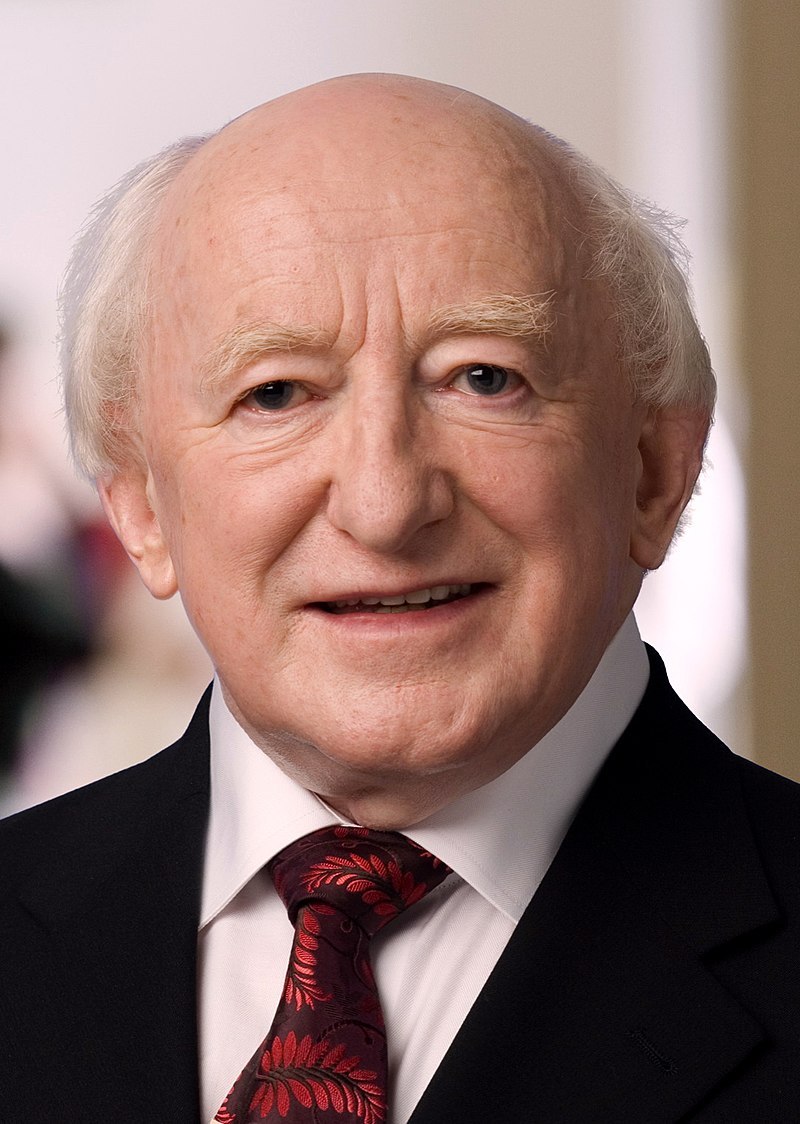
\includegraphics[width=0.2\textwidth]{./images/mickeyd.jpg}
    \caption{Replacement test image used (Michael D. Higgins)}
\end{figure}

\begin{figure}[H]
    \centering
    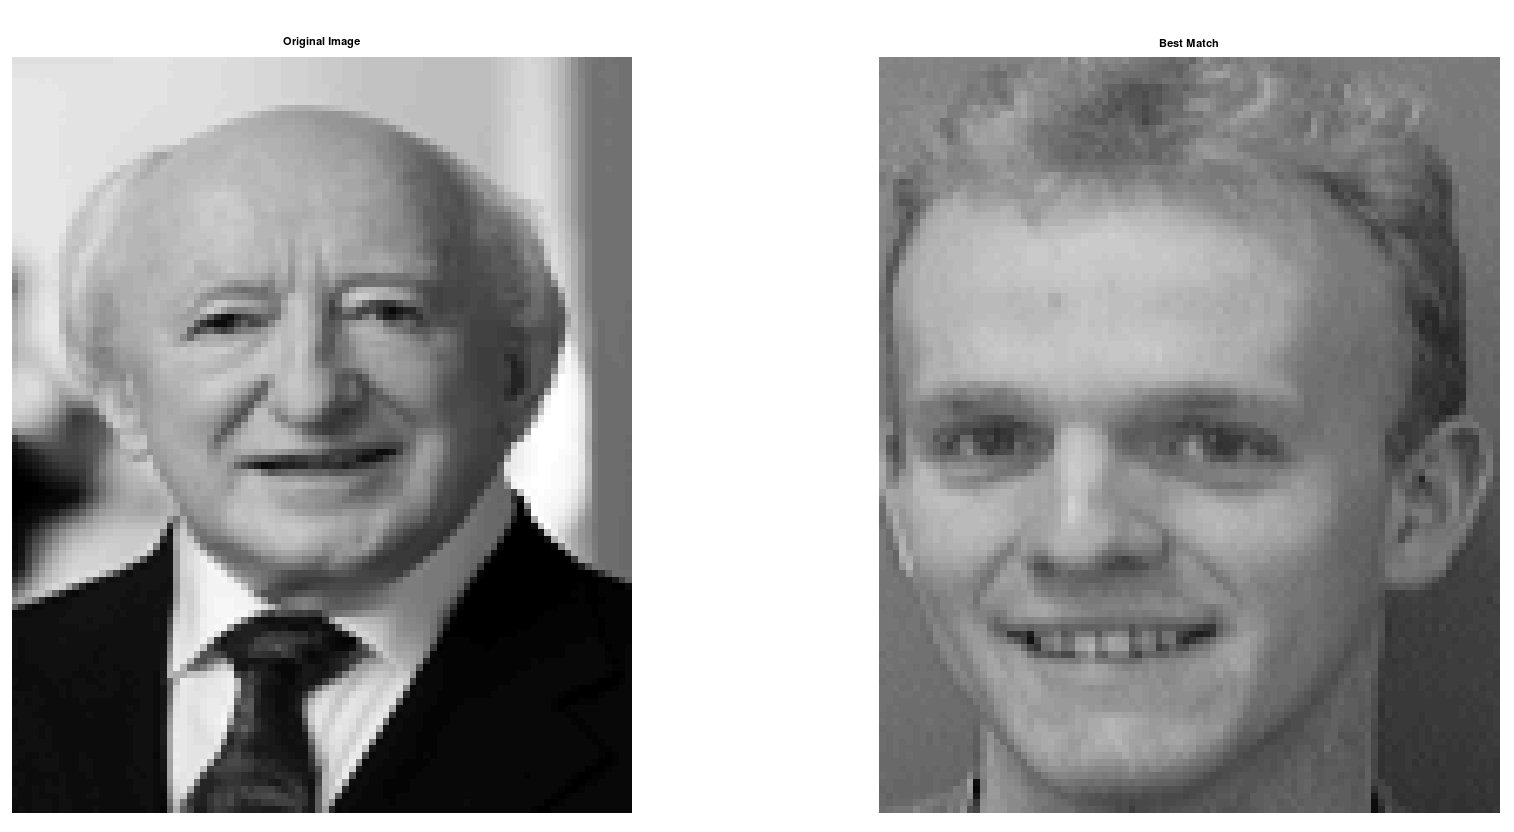
\includegraphics[width=0.8\textwidth]{/home/andrew/currsem/CT404/labs/lab3/latex/images/mickeydlookalike.png}
    \caption{Replacement test image and the best match to it found}
\end{figure}

\section{Effect of Training Images on Accuracy}
% Decrease the number of training images per person from 9 to 5.
% Re-run the code and observe how the accuracy of the test images changes.
% Explain why the accuracy might decrease.
With the original number of training images per person (9), the testing accuracy achieved was 90\%.
\begin{figure}[H]
    \centering
    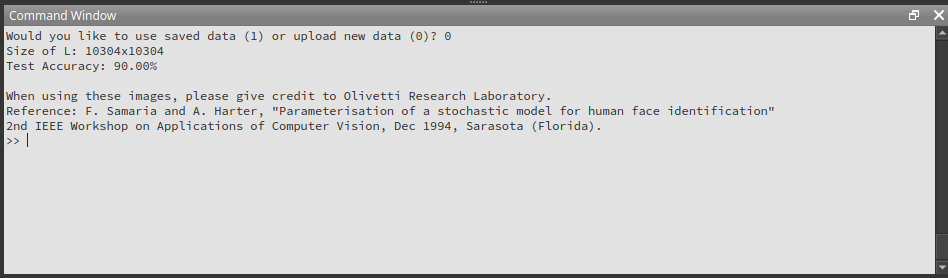
\includegraphics[width=\textwidth]{./images/9trainingimgs.png}
    \caption{Testing accuracy achieved with original number of training images per person (9)}
\end{figure}

To reduce the number of training images used per person, we replaced the following line of code:
\begin{code}
\begin{minted}[firstnumber=16, linenos, breaklines, frame=single]{MATLAB}
train_images_per_subject = 9;  % Number of images per subject for training
\end{minted}
\caption{Original value of \mintinline{matlab}{train_images_per_subject}}
\end{code}

\begin{code}
\begin{minted}[firstnumber=16, linenos, breaklines, frame=single]{MATLAB}
train_images_per_subject = 5;  % Number of images per subject for training
\end{minted}
\caption{Replacement value of \mintinline{matlab}{train_images_per_subject}}
\end{code}

With the reduced number of training images per person (5), the testing accuracy achieved was 85\%.
\begin{figure}[H]
    \centering
    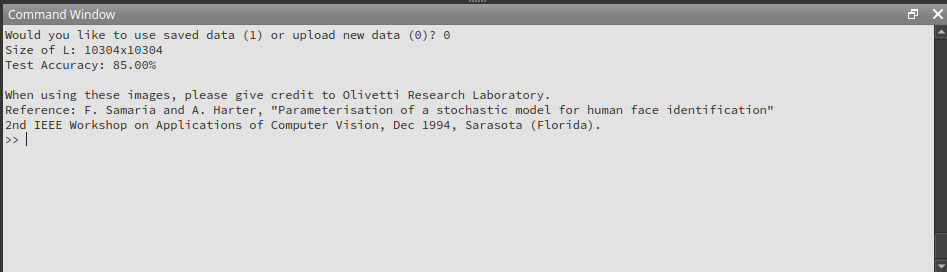
\includegraphics[width=\textwidth]{./images/5trainingimgs.png}
    \caption{Testing accuracy achieved with reduced number of training images per person (5)}
\end{figure}

The reason why the testing accuracy decreased is likely due to reduced feature representation \& dimensional coverage:
fewer training images result in less variability, making it more difficult for the program to capture a comprehensive representation of each face.
The eigenfaces algorithm relies on variance across the training images, and reducing the number of images will reduce the variance captured in the principal components, leading to reduced power to discriminate between different faces.
With fewer examples, there is also a risk of overfitting wherein the mode may fit to the training data too closely and fail to generalise to unseen testing images.

\section{Effect of the Number of Eigenfaces}
% Experiment with different values of $K$, e.g., 40, 200, 300.
% Observe and explain how increasing or decreasing the number of eigenfaces affects the recognition accuracy and the quality of the reconstructed images.

We experimented with different numbers of eigenfaces including 40, 200, \& 300 by assigning different values to \mintinline{matlab}{K} in the following line of code:
\begin{code}
\begin{minted}[firstnumber=16, linenos, breaklines, frame=single]{MATLAB}
K = 200;                   % Number of eigenvectors (Eigenfaces) to use
\end{minted}
\caption{Assigning the value of \mintinline{matlab}{K}}
\end{code}

\begin{figure}[H]
    \centering
    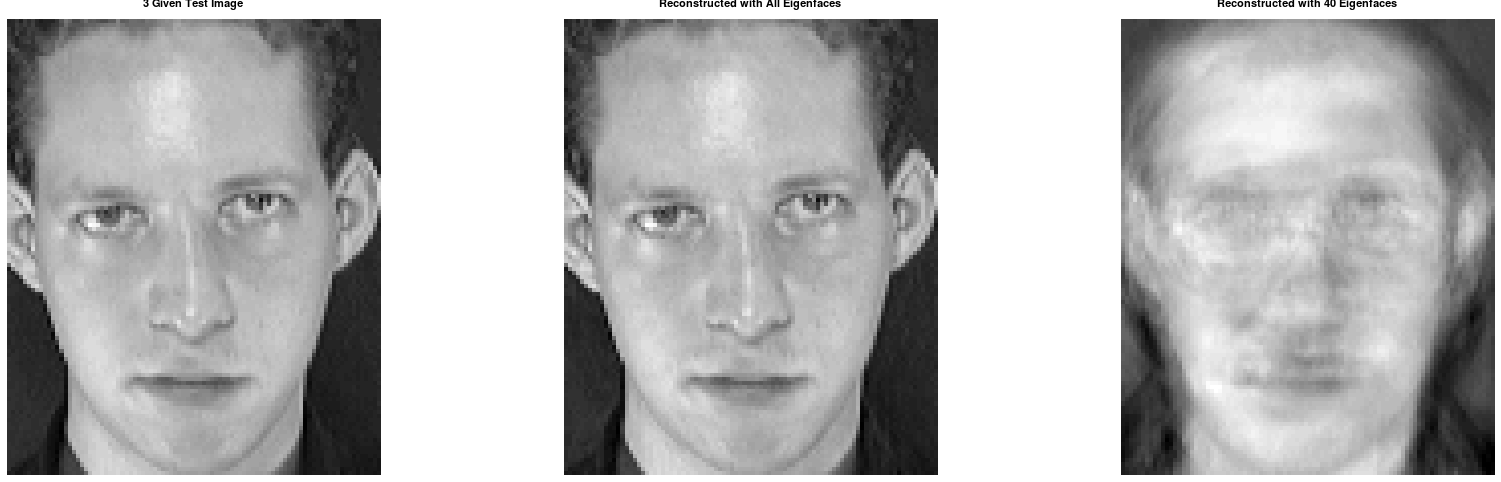
\includegraphics[width=\textwidth]{./images/40acc.png}
    \caption{Reconstructed image achieved with \mintinline{matlab}{K = 40}}
\end{figure}
\begin{figure}[H]
    \centering
    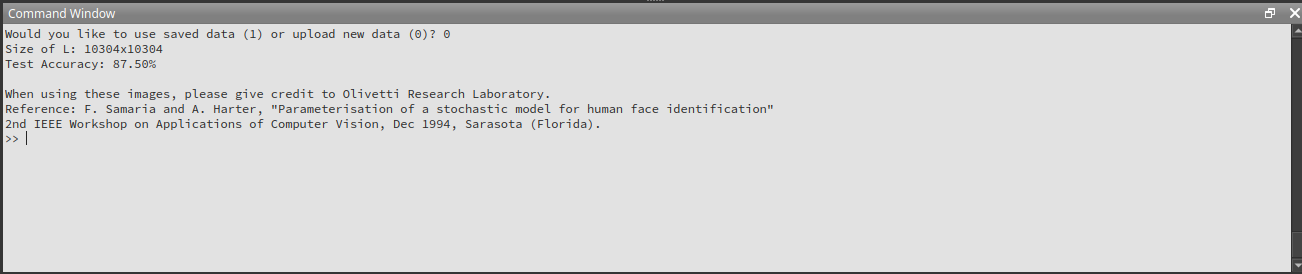
\includegraphics[width=\textwidth]{./images/40rec.png}
    \caption{Testing accuracy achieved with \mintinline{matlab}{K = 40}}
\end{figure}

\begin{figure}[H]
    \centering
    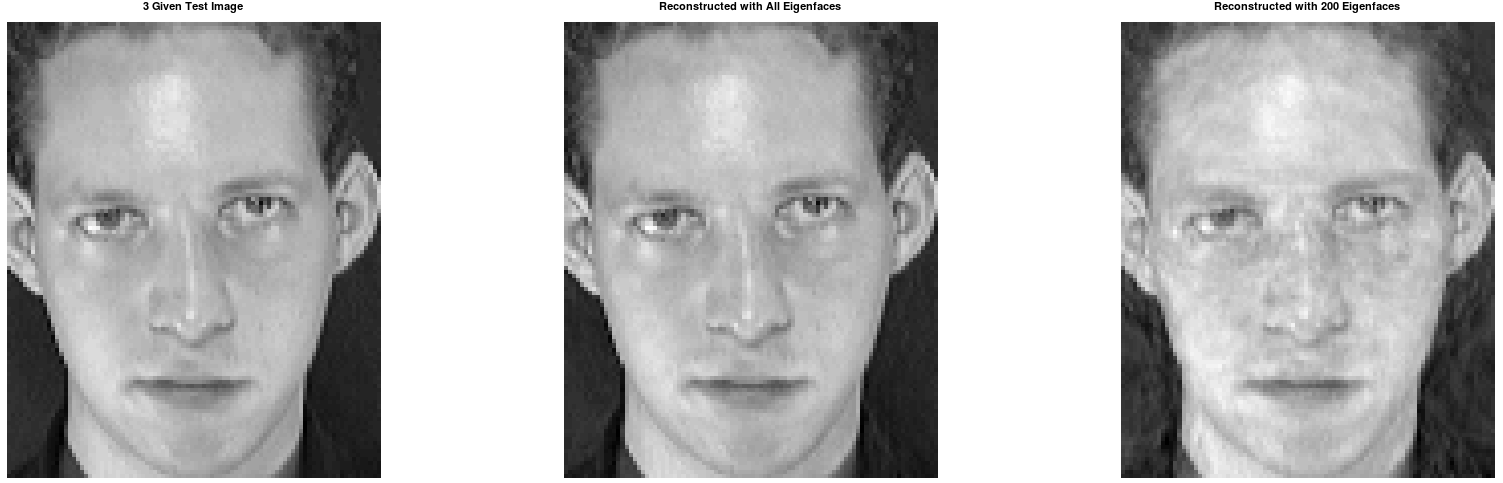
\includegraphics[width=\textwidth]{./images/200rec.png}
    \caption{Reconstructed image achieved with \mintinline{matlab}{K = 200}}
\end{figure}
\begin{figure}[H]
    \centering
    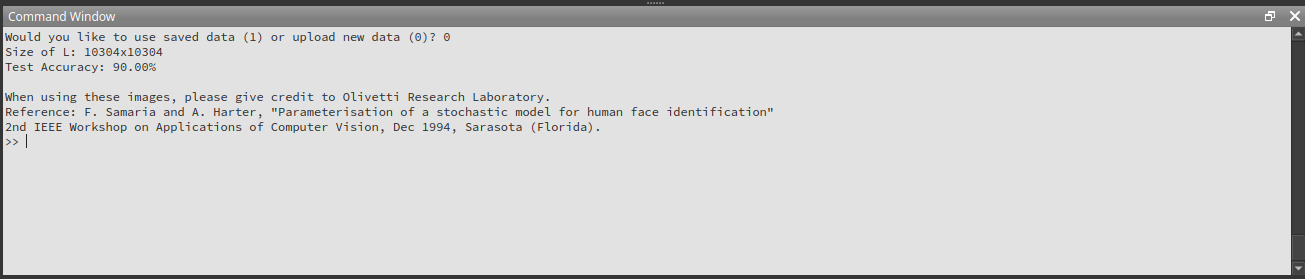
\includegraphics[width=\textwidth]{./images/200acc.png}
    \caption{Testing accuracy achieved with \mintinline{matlab}{K = 200}}
\end{figure}

\begin{figure}[H]
    \centering
    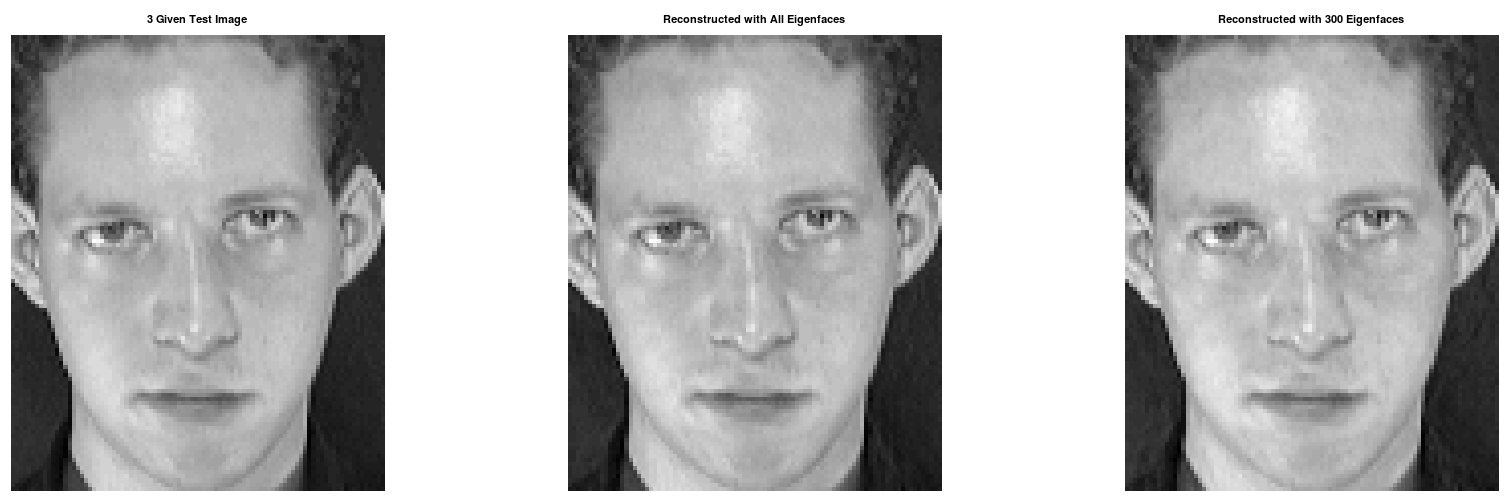
\includegraphics[width=\textwidth]{./images/300rec.png}
    \caption{Reconstructed image achieved with \mintinline{matlab}{K = 300}}
\end{figure}
\begin{figure}[H]
    \centering
    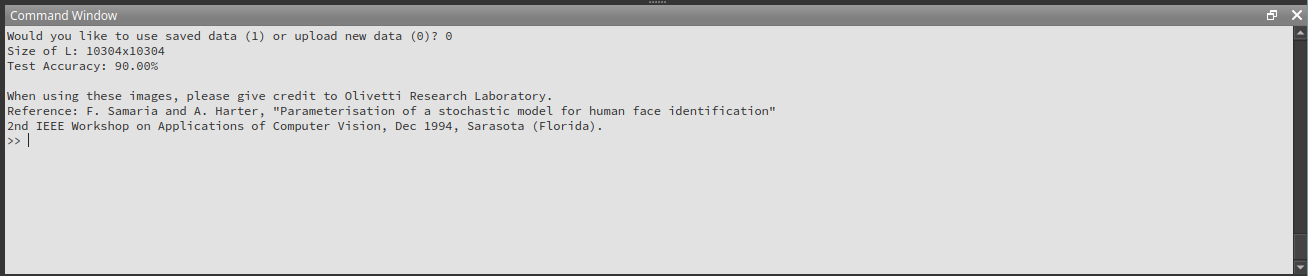
\includegraphics[width=\textwidth]{./images/300acc.png}
    \caption{Testing accuracy achieved with \mintinline{matlab}{K = 300}}
\end{figure}

We observed that the quality of the reconstructed images appeared to scale with the number of eigenfaces used:
the reconstructed image achieved with \mintinline{matlab}{K = 40} was barely recognisable as human face, the reconstructed image achieved with \mintinline{matlab}{K = 200} was far better but had quite a lot of blur \& noise, and the reconstructed image achieved with \mintinline{matlab}{K = 300} was better again with reduced blur \& noise.
Interestingly, despite the marked improvement in the reconstructed images, the testing accuracy was not greatly affected:
\mintinline{matlab}{K = 40} achieved a testing accuracy of 87.50\%, \mintinline{matlab}{K = 200} achieved a slightly improved testing accuracy of 90\%, and \mintinline{matlab}{K = 300} failed to improve on this and also achieved a testing accuracy of 90\%.
\\\\
The low testing accuracy with \mintinline{matlab}{K = 40} can be explained by there being insufficient eigenfaces to capture the all the relevant facial features.
We can see that the features were better-captured with \mintinline{matlab}{K = 200}, and we observed that the improvement plateaued here as \mintinline{matlab}{K = 300} failed to improve the testing accuracy.
This indicates that \mintinline{matlab}{K = 200} was sufficient to capture the relevant features.

\section{Adding Your Friend's Faces}
To add the images of the 5 new people to the dataset, we took 10 images of each person and added them to directories in the data directory named \verb|s41| through \verb|s45|.
Because each image we had was either JPEG or PNG and the program relies on files being named \mintinline{matlab}{%d.pgm} where \mintinline{matlab}{%d} is some integer, we had to convert and re-name all the files for each person.
As one of us was using a Linux system, we achieved this using a one-line shell script on the command line using a program called ImageMagick:
\begin{code}
\begin{minted}[ linenos, breaklines, frame=single]{shell}
count=1; for file in *; do magick "$file" "$count.pgm"; ((count++)); rm "$file"; done 
\end{minted}
\caption{Script used to rename \& convert image files}
\end{code}

We then realised that the images had to be re-sized to work with the program as well, so we ran the following script to resize the images:
\begin{code}
\begin{minted}[ linenos, breaklines, frame=single]{shell}
for file in *; do magick $file -resize 92x112! $file; done 
\end{minted}
\caption{Script used to rename \& convert image files}
\end{code}

We then edited the code to reflect the new number of subjects:
\begin{code}
\begin{minted}[firstnumber = 15, linenos, breaklines, frame=single]{matlab}
num_subjects = 45;        % Number of subjects in the dataset
\end{minted}
\caption{Updated number of subjects}
\end{code}

\begin{figure}[H]
    \centering
    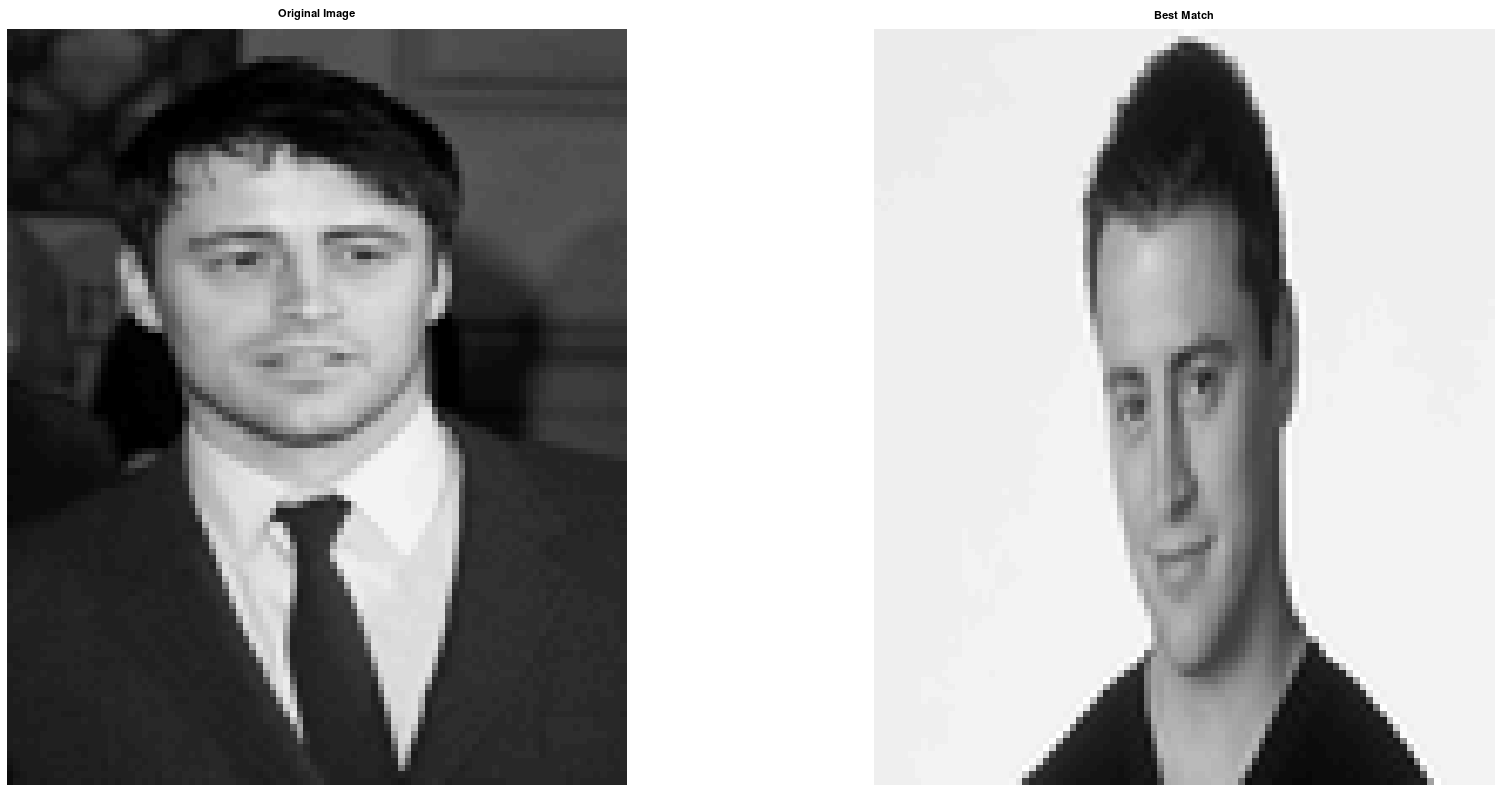
\includegraphics[width=\textwidth]{./images/fwend.png}
    \caption{ Best match found for unseen friend picture }
\end{figure}

The model recognised the new photograph of our friend very well, correctly matching the unseen test image with a training image of the same individual! 




\end{document}
